\documentclass[12pt]{amsart}
\usepackage[margin=3cm]{geometry}                % See geometry.pdf to learn the layout options. There are lots.
\geometry{letterpaper}                   % ... or a4paper or a5paper or ... 
%\geometry{landscape}                % Activate for for rotated page geometry
%\usepackage[parfill]{parskip}    % Activate to begin paragraphs with an empty line rather than an indent
\usepackage{graphicx}
\usepackage{amssymb}
\usepackage{epstopdf}
\DeclareGraphicsRule{.tif}{png}{.png}{`convert #1 `dirname #1`/`basename #1 .tif`.png}

\title{Coupled Pendulums}
\author{Caspar Lant}
                                         

\begin{document}
\maketitle
	
\pagebreak
\textbf{The Objective} of this week's experiment is to explore the interactions of two pendulums which share a common axis, as a way to frame our studies of waves and harmonic motion.\\\\
\textbf{Theoretical Background/Abstract: }
\paragraph{Way back in the mid 17th century, the brilliant Huygens noticed that the two grandfather clocks on his mantlepiece (who keeps two grandfather clocks on their mantlepiece?)  had fallen into synchrony! The pendulums that drove the two clocks were not oscillating in phase, as one might expect, but 180� out of phase. We will learn later that this is one of 2 normal modes that exist for a two-pendulum oscillating system. From here, Huygens formulated an equation that could generalize the motion of two pendulums. Before this, let's assume the following conditions, which give rise to force equations for each pendulum}
\paragraph{\\Let's assume that $l$ and $m$ are the same for each pendulum, that each pendulum oscillates in the same plane, angles are small;  $ sin\theta \approx \theta, $ and that $F_a = - Kl(\theta_a- \theta_b), $ $F_b = - Kl(\theta_a- \theta_b)$, $\Sigma F = 0$}

\begin{equation}
ml \frac{d^2\theta_a}{dt^2} = -mg\theta_a - Kl_0 (\theta_a- \theta_b)
\end{equation}
\begin{equation}
\frac{d^2\theta_a}{dt^2}  + \frac{g}{l}\theta_a + K \frac{l_0}{ml} (\theta_a- \theta_b) = 0 ?
\end{equation}
\begin{equation}
\frac{d^2\theta_a}{dt^2}  + \omega^2 \theta_a + C (\theta_a- \theta_b) = 0 \\
\Big(\omega_0 = \sqrt{\frac{g}{l}}\Big)
\end{equation}
\paragraph{Where $l_0$ is the position of the spring coupling between the pendulums, with $l_0 = 0$ at the axis of oscillation}
\paragraph{\\Normal modes denote starting conditions under which the motion of the pendulum is stable, and constant in phase-space. This is to say that, if you start a two pendulum in one of its two normal modes, it will continue to oscillate in this mode, with no energy trade-off between the pendulums. These modes are eigenvectors of the equation to follow. The so-called ``slow mode'' is given by the initial condition $\theta_a = \theta_b$, and is shown in vector-form by $[1,1]$. The second, ``fast mode'' is given by $\theta_a = -\theta_b$, or $[1,-1]$}

\paragraph{\\For arrangements of pendulums that cannot be classified as either of the the system's two normal modes, we find the following equation:\\}

\begin{equation}
\vec{X}(t) = \left[\begin{array}{c}1 \\1\end{array}\right](a_{1}cos\omega_{1}t+ b_{1}sin\omega_{1}t) + 
\left[\begin{array}{c}1 \\-1\end{array}\right](a_{2}cos\omega_{2}t+ b_{2}sin\omega_{2}t)
\end{equation}

\newpage
\begin{figure}[ht!]
\centering
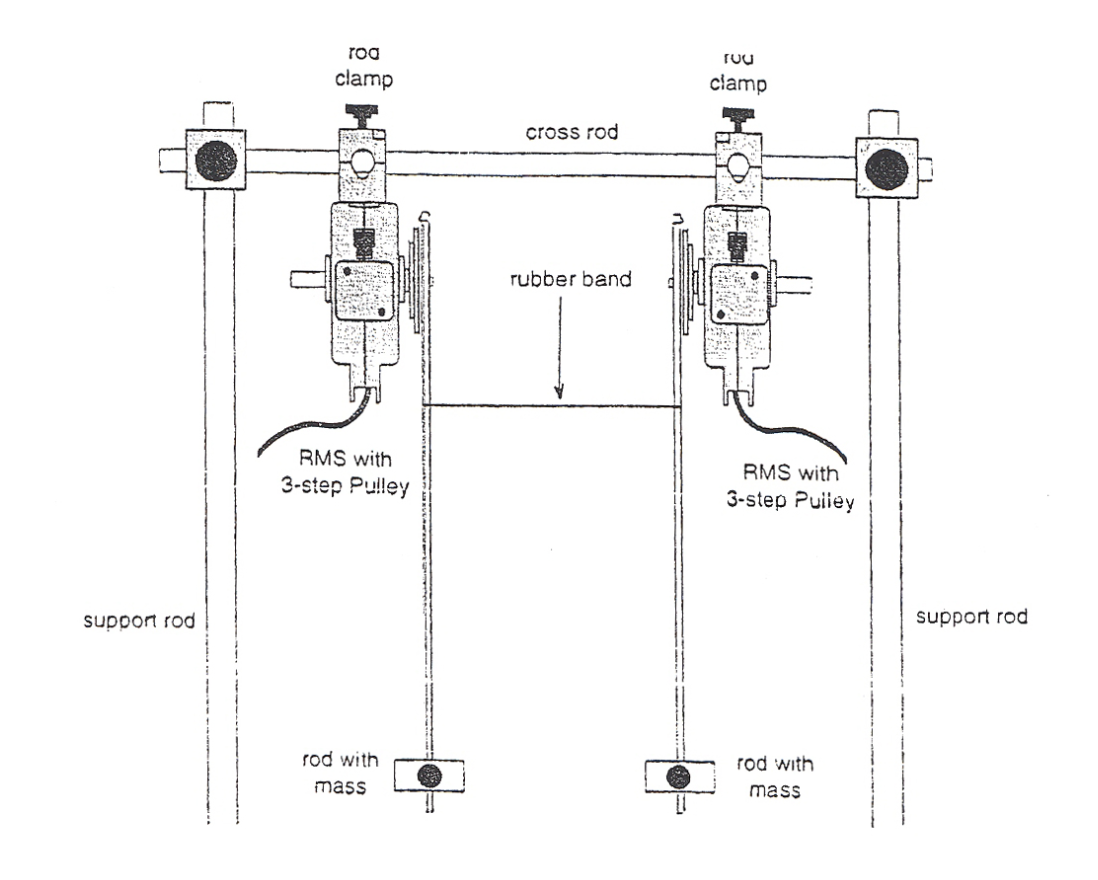
\includegraphics[width=100mm]{Figure.png}
\caption{Experimental Setup}
\end{figure}
\medspace
\textbf{Experimental Procedure}?
\smallspace
\begin{itemize}
\item Set up the two pendulum system in the manner detailed by the above diagram.
\item Connect the two rotary distance sensors to Data Studio via the provided interface.
\item Create a display in Data Studio that graphs the position of each distance sensor over time.
\item Match the frequency of one pendulum to that of its partner by adjusting the position of its mass. It's of note here that we disregard the mass of the rod in our calculations. 
\item Plot the oscillation of each pendulum in Data Studio and compute its frequency with a best-fit sine function.
\item Connect the rubber band to each pendulum at a distance of 5cm.
\item Start the pendulums off in the ``slow mode'' and record their oscillations in Data Studio. 
\item Do the same for the ``fast mode''.
\item Now for something more interesting: start the pendulum off in a ``non-normal'' mode by displacing one pendulum and keeping the other at zero position. Ensure the the angle of displacement is sufficiently small, in accordance with the paraxial approximation on page one.
\item Repeat each experiment for rubber band length distances 10cm, 15cm, 20cm, and so on. How does the position of the rubber band affect the rate of the pendulums' oscillation?
\end{itemize}

\begin{figure}[ht!]
\centering
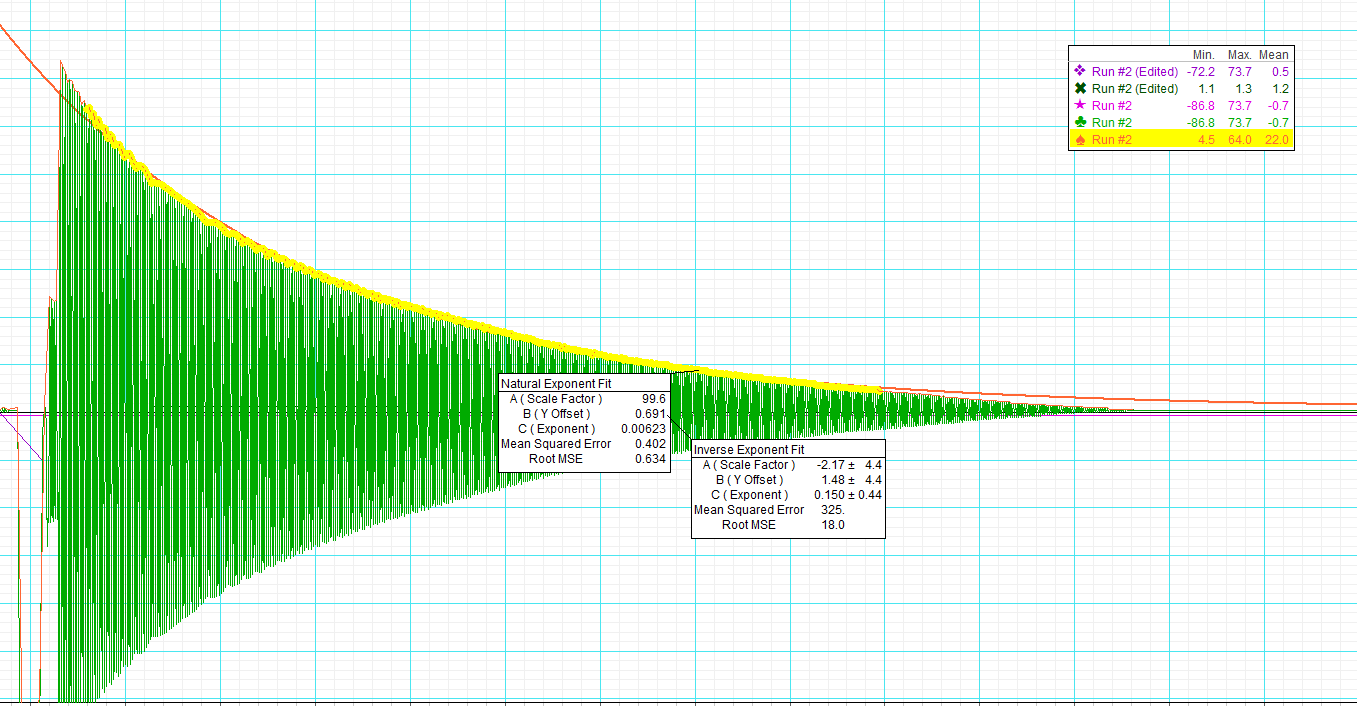
\includegraphics[width=160mm]{Capture.PNG}
\caption{Extra Credit: Calculating the Damping of a Single Pendulum $$Damping Curve: 97e^{-0.00594t}, \gamma = 0.00594$$}
\end{figure}

\begin{figure}[ht!]
\centering
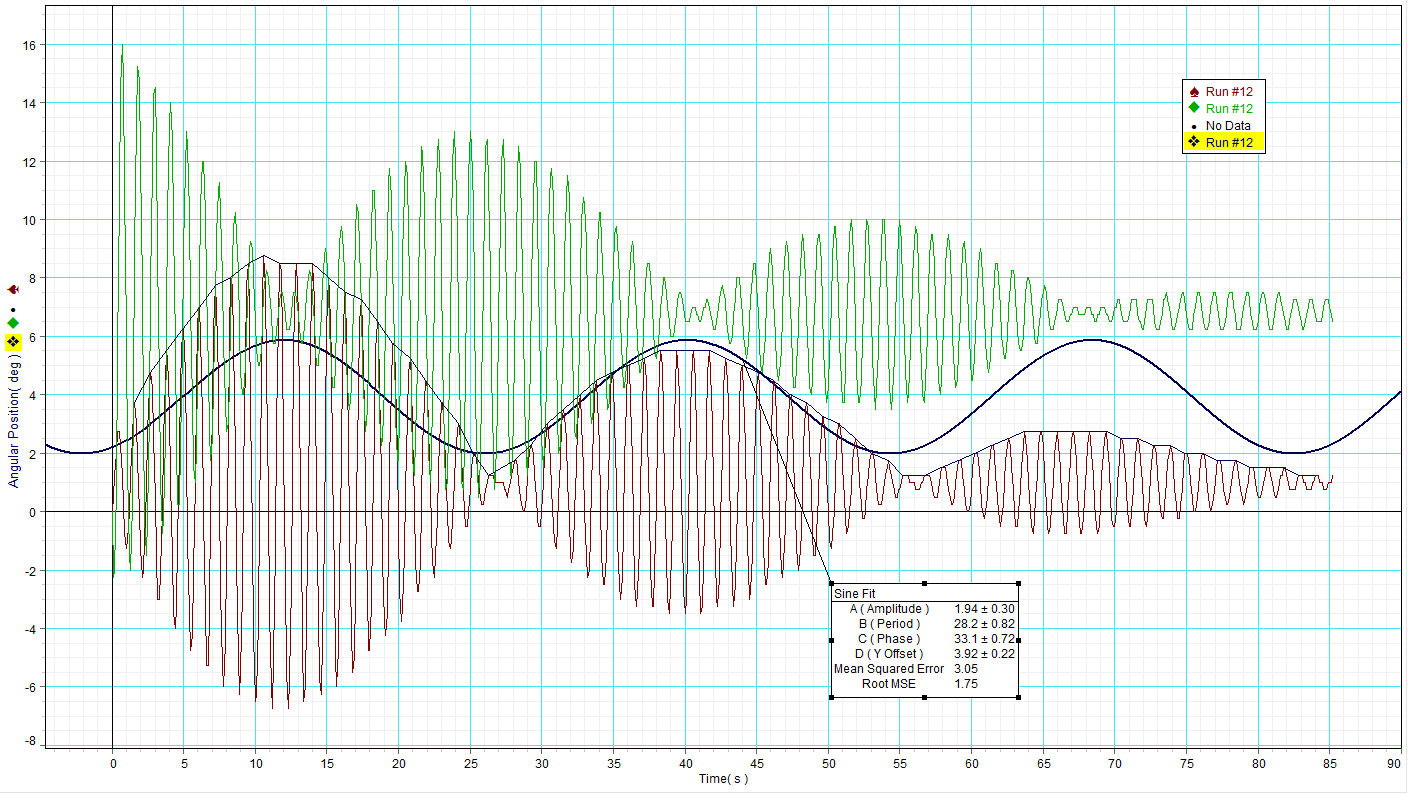
\includegraphics[width=160mm]{Capture1.PNG}
\caption{Harmonic Resonance of two Pendulums}
\end{figure}

\begin{table}[]
\centering
\caption{Experimental Data}
\label{my-label}
\begin{tabular}{llllll}
Pend Mass (g) & Rubber Band Height (cm) & $\omega_b$ & $\omega_{av}$ & $\omega_1$ & $\omega_2$ \\
74.4          & 5                       & 0.018      & 0.901         & 0.855      & 0.893      \\
74.4          & 10                      & 0.060      & 0.990         & 0.862      & 1.000      \\
74.4          & 20                      & 0.380      & 0.862         & 0.862      & 1.403     
\end{tabular}
\end{table}
\smallskip
\begin{table}[]
\centering
\caption{Theoretical Calculations}
\label{my-label}
\begin{tabular}{llllll}
{Pend Mass (g)} & {Rubber Band Height (cm)} & \textbf{$\omega_b$} & \textbf{$\omega_{av}$} & \textbf{$\omega_1$} & \textbf{$\omega_2$} \\
74.4                   & 5                                & 0.019               & 0.874                  & 0.855               & 0.893               \\
74.4                   & 10                               & 0.069               & 0.931                  & 0.862               & 1.000               \\
74.4                   & 20                               & 0.270               & 1.132                  & 0.862               & 1.403              
\end{tabular}
\end{table}
hello
\vfill
\LaTeX
\end{document} 